\documentclass{article}
\usepackage{graphicx}
\title{%
  Searching a Graph \\
  \large with Hillclimbing and Simulated Annealing}
\author{Brendan Waters}
\date{March 20, 2016}
\begin{document}
  \maketitle
  Out of the three searches, hillclimbing is the least accurate. Since there are many local extrema in the given function this algorithm very rarely gets close to the global minimum. As shown in Figure 1, if this algorithm starts at the corner of the given domain it only travels a short distance before it gets stuck at a local minimum. The value found by this hillclimb with a step size of 0.01 is z = -0.082336 at the coordinates (2.49, 2.40). This is pretty far off from the global minimum which is approximately z = -0.150271 and occurs at approximate (+/-2.1729, 0).
  \par
  Repeating hillclimbing by restarting at random places greatly increases the accuracy of the search. By doing this with enough restarts, at least one of the hillclimbs will reach the global minimum or at least get very close. I did this search using a step size of 0.01 with 500 random restarts shown in Figure 2. The result of this specific search was approximately z = -0.150271 occuring at approximately (-2.172862, -0.001040) which is very close to the global minimum.
  \par
  Simulated Annealing is also very accurate, as long as the temperature decreases slowly enough. I ran simulated annealing with a max temperature of 100 with the temperature decreasing by 1 percent with each cycle until it is less than 0.00001 as it approaches 0. In addition, my algorithm attempts to make 50 random moves at each temperature. The value of the search shown in Figure 3 was approximately z = -0.150179 occuring at approximately (2.179588, -0.005372). This is also very close to one of the two global minima.
  \par
  These algorithms also vary in the amount of time they take to complete with hillclimbing being by far the fastest. This is because a single hillclimb does very few calclulations, searching only a very small portion of the space which is what also leads to its inaccuracy. Both simulated annealing and hillclimbing with random restarts can take a very long time depending on their parameters. This is because the more restarts are done or the slower the temperature is lowered, the larger the amount of search space the algorithm explores until it effectively visits every point in the space. However, these algorithms can usually find the global extrema without actually having to search the entire space so it is up to the user to determine efficient parameters which give both an accurate and speedy result.
  \begin{figure}
    \makebox[\textwidth][c]{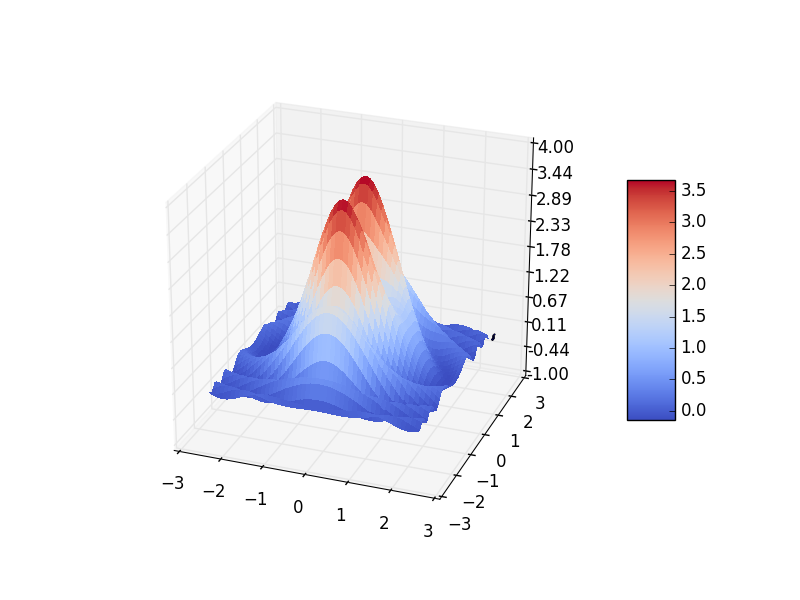
\includegraphics[width=1.5\textwidth]{hillclimb.png}}%
    \caption{Hillcimbing Path Starting From (2.5, 2.5)}
  \end{figure}
  \begin{figure}
    \makebox[\textwidth][c]{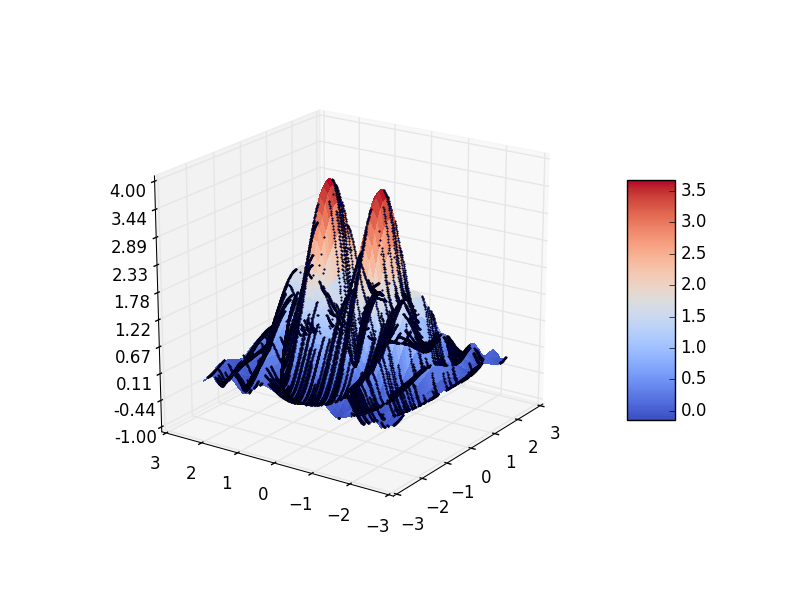
\includegraphics[width=1.5\textwidth]{randomrestarts.png}}%
    \caption{Hillclimbing with 500 Random Restarts}
  \end{figure}
  \begin{figure}
    \makebox[\textwidth][c]{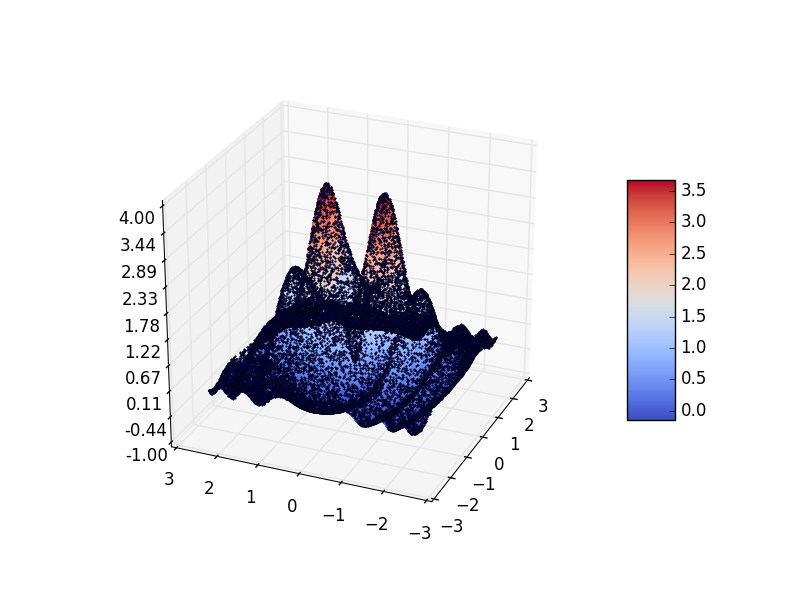
\includegraphics[width=1.5\textwidth]{simulatedannealing.png}}%
    \caption{Simulated Annealing With Maximum Temperature of 100}
  \end{figure}
\end{document}
